\chapter{Basic usage}
\label{chap:Basic usage}

\section{Conventions}
\label{sec:Conventions}

All classes that are accessible to users are within the name space
\cppinline{vsmc}. Class names are in \cppinline{CamelCase} and function names,
free or class methods, are in \cppinline{small_cases}. In the remaining of this
guide, we will omit the \cppinline{vsmc::} name space qualifiers. We will use
``function'' for referring to name space scope functions and ``method'' for
class member functions.

\section{Getting and installing the library}
\label{sec:Getting and installing the library}

The library is hosted at
GitHub\footnote{\url{https://github.com/zhouyan/vSMC}}. This is a header only
\cpp template library. To install the library just move the contents of the
\texttt{include} directory into a proper place, e.g.,
\texttt{/usr/local/include} on Unix-alike systems. This library requires
working \cppoo, \blas and \lapack implementations. Standard C interface headers
for the later two (\cppinline{cblas.h} and \cppinline{lapacke.h}) are required.
Intel Threading Building
Blocks\footnote{\url{https://www.threadingbuildingblocks.org}} (\tbb), Intel
Math Kernel Library\footnote{\url{https://software.intel.com/en-us/intel-mkl}}
(\mkl) and \hdf\footnote{\url{http://www.hdfgroup.org}} are optional
third-party libraries. One need to define the configuration macros
\cppinline{VSMC_HAS_TBB}, \cppinline{VSMC_HAS_MKL} and
\cppinline{VSMC_HAS_HDF5} to nonzero values before including any \vsmc headers
to make their existence known to the library, respectively.

\section{Concepts}
\label{sec:Concepts}

The library is structured around a few core concepts. A sampler is responsible
for running an algorithm. It is composed by a particle system and operations on
it. A particle system is formed by the states $\{X^{(i)}\}_{i=1}^N$ and weights
$\{W^{(i)}\}_{i=1}^N$. This system will also be responsible for resampling. All
user defined operations are to be applied to the whole system. These are
``initialization'' and ``moves'' which are applied before resampling, and
``\mcmc'' moves which are applied after resampling. These operations do not
have to be \mcmc kernels. They can be used for any purpose that suits the
particular algorithm. Most statistical inferences requires calculation of
$\sum_{i=1}^NW^{(i)}\varphi(X^{(i)})$ for some function $\varphi$. This can be
carried out along each sampler iteration by a monitor. Table~\ref{tab:concepts}
lists these concepts and the corresponding classes in the library. Each of them
are introduced in detail in the following sections.

\begin{table}[t]
  \begin{tabu}{X[l]X[2l]}
    \toprule
    Concept & Class \\
    \midrule
    State, $\{X^{(i)}\}_{i=1}^N$            & \texttt{T}, user defined   \\
    Weight, $\{W^{(i)}\}_{i=1}^N$           & \texttt{Weight}            \\
    Particle, $\{W^{(i)},X^{(i)}\}_{i=1}^N$ & \texttt{Particle<T>}       \\
    Single particle, $\{W^{(i)},X^{(i)}\}$  & \texttt{SingleParticle<T>} \\
    Sampler        & \texttt{Sampler<T>}                           \\
    Initialization & \texttt{Sampler<T>::init\_type}, user defined \\
    Move           & \texttt{Sampler<T>::move\_type}, user defined \\
    \mcmc          & \texttt{Sampler<T>::mcmc\_type}, user defined \\
    Monitor        & \texttt{Monitor<T>}                           \\
    \bottomrule
  \end{tabu}
  \caption{Core concepts of the library}
  \label{tab:concepts}
\end{table}

\subsection{State}
\label{sub:State}

The library gives users the maximum flexibility of how the states
$\{X^{(i)}\}_{i=1}^N$ shall be stored and structured. Any class type with a
constructor that takes a single integer value, the number of particles, as its
argument, and a method named \cppinline{copy} is acceptable. For example,
\begin{cppcode*}{texcomments}
  class T
  {
      public:
      T(std::size_t N);

      template <typename IntType>
      void copy(std::size_t N, IntType *index)
      {
          for (std::size_t i = 0; i != N; ++i) {
              // Let $a_i =$ index[i], set $X^{(i)} = X^{(a_i)}$
          }
      }
  };
\end{cppcode*}
How the state values are actually stored and accessed are entirely up to the
user. The method \cppinline{copy} is necessary since the library assumes no
knowledge of the internal structure of the state. And thus it cannot perform
the last step of a resampling algorithm, which makes copies of particles with
larger weights and eliminate those with smaller weights.

For most applications, the values can be stored within an $N$ by $d$ matrix,
where $d$ is the dimension of the state. The library provides a convenient
class template for this situation,
\begin{cppcode}
  template <MatrixLayout Layout, std::size_t Dim, typename T>
  class StateMatrix;
\end{cppcode}
where \cppinline{Layout} is either \cppinline{RowMajor} or
\cppinline{ColMajor}, which specifies the matrix storage layout;
\cppinline{Dim} is a non-negative integer value. If \cppinline{Dim} is zero,
then the dimension may be changed at runtime. If it is positive, then the
dimension is fixed and cannot be changed at runtime. The last template
parameter \cppinline{T} is the \cpp type of state space. The following
constructs an object of this class,
\begin{cppcode}
  StateMatrix<ColMajor, Dynamic, double> s(N);
\end{cppcode}
where \cppinline{Dynamic} is just an enumerator with value zero. We can specify
the dimension at runtime through the method \cppinline{s.resize_dim(d)}. Note
that, if the template parameter \cppinline{Dim} is positive, then this call
results in a compile-time error.

To access $X_{ij}$, the value of the state of the $i$\ith particle at the
$j$\ith coordinate, one can use the method \cppinline{s.state(i,j)}. The method
\cppinline{s.data()} returns a pointer to the beginning of the matrix.  If
\cppinline{Layout} is \cppinline{RowMajor}, then the method
\cppinline{s.row_data(i)} returns a pointer to the beginning of the $i$\ith
row. If \cppinline{Layout} is \cppinline{ColMajor}, then the method
\cppinline{s.col_data(j)} returns a pointer to the beginning of the $j$\ith
column. These methods help interfacing with numerical libraries, such as \blas.

The \cppinline{StateMatrix} class deliberately does not provide a
\cppinline{resize} method. There are algorithms that change the sample size
between iterations. However, such algorithms often change size through
resampling or other methods, either deterministically or stochastically. An
example of changing size of a sampler is provided in section~\ref{sec:Resizing
  a sampler}.

\subsection{Weight}
\label{sub:Weight}

The vector of weights $\{W^{(i)}\}_{i=1}^N$ is abstracted in the library by the
\cppinline{Weight} class. The following constructs an object of this class,
\begin{cppcode}
  Weight w(N);
\end{cppcode}
There are a few methods for accessing the weights,
\begin{cppcode*}{texcomments}
  w.ess();          // Get {\normalfont\textsc{ess}}
  w.set_equal();    // Set $W^{(i)} = 1/N$
\end{cppcode*}
The weights can be manipulated, given a vector of length $N$, say $v$,
\begin{cppcode*}{texcomments}
  w.set(v);         // Set $W^{(i)} \propto v^{(i)}$
  w.mul(v);         // Set $W^{(i)} \propto W^{(i)} v^{(i)}$
  w.set_log(v);     // Set $\log W^{(i)} = v^{(i)} + \text{const.}$
  w.add_log(v);     // Set $\log W^{(i)} = \log W^{(i)} + v^{(i)} + \text{const.}$
\end{cppcode*}
The method \cppinline{w.data()} returns a pointer to the normalized weights. It
is important to note that the weights are always normalized and all mutable
methods only allow access to $\{W^{(i)}\}_{i=1}^N$ as a whole.

\subsection{Particle}
\label{sub:Particle}

A particle system is composed of both the state values, which is of user
defined type, say \cppinline{T}, and the weights. The following constructs an
object of class \cppinline{Particle<T>},
\begin{cppcode}
  Particle<T> particle(N);
\end{cppcode}
The method \cppinline{particle.value()} returns the type \cppinline{T} object,
and \cppinline{particle.weight()} returns the type \cppinline{Weight}
object\footnote{More precisely, it is a \cppinline{Particle<T>::weight_type}
  object, whose exact type depends on the type \cppinline{T}. See
  section~\ref{sec:Customizing member types} for more details. If the user does
  not do something special as shown in that section, then the default type is
  the class \cppinline{Weight}}. They are constructed with the same integer
value $N$ when the above constructor is invoked.

As a Monte Carlo algorithm, random number generators (\rng) will be used
frequently. The user is free to use whatever \rng mechanism as they see fit.
However, one common issue encountered in practice is how to maintain
independence of the \rng streams between function calls. For example, consider
below a function that manipulates some state values,
\begin{cppcode}
  void function(double &x)
  {
      std::mt19937 rng;
      std::normal_distribution<double> rnorm(0, 1);
      x = rnorm(rng);
  }
\end{cppcode}
Every call of this function will give \cppinline{x} exactly the same value.
This is hardly what the user intended. One might consider an global \rng or one
as class member data. For example,
\begin{cppcode}
  std::mt19937 rng;
  void function(double &x)
  {
      std::normal_distribution<double> rnorm(0, 1);
      x = rnorm(rng);
  }
\end{cppcode}
This will work fine as long as the function is never called by two threads at
the same time. However, \smc algorithms are natural candidates to
parallelization. Therefore, the user will need to either lock the \rng, which
degenerates the performance, or construct different \rng{}s for different
threads. The later, though ensures thread-safety, has other issues. For
example, consider
\begin{cppcode*}{texcomments}
  std::mt19937 rng1(s1); // For thread $i_1$ with seed $s_1$
  std::mt19937 rng2(s2); // For thread $i_2$ with seed $s_2$
\end{cppcode*}
where the seeds $s_1 \ne s_2$. It is difficult to ensure that the two streams
generated by the two \rng{}s are independent. Common practice for parallel \rng
is to use sub-streams or leap-frog algorithms. Without going into any further
details, it is sufficient to say that this is perhaps not a problem that most
users bother to solve.

The library provides a simple solution to this issue. The method
\cppinline{particle.rng(i)} returns a reference to an \rng that conforms to the
\cppoo uniform \rng concept. It can be called from different threads at the
same time, for example,
\begin{cppcode*}{texcomments}
  auto &rng1 = particle.rng(i1); // Called from thread $i_1$
  auto &rng2 = particle.rng(i2); // Called from thread $i_2$
\end{cppcode*}
If $i_1 \ne i_2$, then the subsequent use of the two \rng{}s are guaranteed to
be thread-safe. In addition, they will produce independent streams. If \tbb is
available to the library, then it is also thread-safe even if $i_1 = i_2$. One
can write functions that process each particle, for example,
\begin{cppcode*}{texcomments}
  void function(std::size_t i)
  {
      auto &rng = particle.rng(i);
      // Process the $i$\textsups{t{}h} particle using rng
  }
\end{cppcode*}
And if later this function is called from a parallelized environment, it is
still thread-safe and produce desired statistical results. The details of the
\rng system are documented later in chapter~\ref{chap:Random number generating}.

\subsection{Single particle}
\label{sub:Single particle}

It is often easier to define a function $f(X^{(i)})$ than
$f(X^{(1)},\dots,X^{(N)})$. However, \cppinline{Particle<T>} only provides
access to $\{X^{(i)}\}_{i=1}^N$ as a whole through
\cppinline{particle.value()}. To allow direct access to $X^{(i)}$, the library
uses a class template \cppinline{SingeParticle<T>}. An object of this class is
constructed from the index $i$ of the particle, and a pointer to the particle
system it belongs to,
\begin{cppcode}
  SingleParticle<T> sp(i, &particle);
\end{cppcode}
or more conveniently,
\begin{cppcode}
  auto sp = particle.sp(i);
\end{cppcode}
In its most basic form, it has the following methods,
\begin{cppcode}
  sp.id();       // Get the value i that sp was constructed with
  sp.particle(); // Get a reference to the Particle<T> object sp belongs to
  sp.rng();      // => sp.particle().rng(sp.id());
\end{cppcode}
If \cppinline{T} is a subclass of \cppinline{StateMatrix}, then it has two
additional methods,
\begin{cppcode}
  sp.dim();    // => sp.particle().value().dim();
  sp.state(j); // => sp.particle().value().state(sp.id(), j);
\end{cppcode}
It is clear now that the interface of \cppinline{SingleParticle<T>} depends on
the type \cppinline{T}. Later in section~\ref{sec:Extending SP}
we will show how to insert additional methods into this class.

A \cppinline{SingleParticle<T>} object is similar to an iterator. In fact, it
supports almost all of the operations of a random access iterator with two
exceptions. First dereferencing a \cppinline{SingleParticle<T>} object returns
itself. The support of \cppinline{operator*} allows the range-based for loop to
be applied on a \cppinline{Particle<T>} object, for example,
\begin{cppcode}
  for (auto sp : particle) {
      // sp is of type SingleParticle<T>
  }
\end{cppcode}
The above loop does make some sense. However trying to dereferencing a
\cppinline{SingleParticle<T>} object in other contexts does not make much
sense. Recall that it is an \emph{index}, not a \emph{pointer}. The library
does not require the user defined type \cppinline{T} to provide access to
individual values, and thus it cannot dereference a
\cppinline{SingleParticle<T>} object to obtain such a value. Similarly, the
expression \cppinline{sp[n]} returns \cppinline{sp + n}, another
\cppinline{SingleParticle<T>} object. For the same reason,
\cppinline{operator->} is not supported at all.

\subsection{Sampler}
\label{sub:Sampler}

A sampler can be constructed in a few ways,
\begin{cppcode}
  Sampler<T> sampler(N);
\end{cppcode}
constructs a sampler that is never resampled, while
\begin{cppcode}
  Sampler<T> sampler(N, Multinomial);
\end{cppcode}
constructs a sampler that is resampled every iteration, using the multinomial
algorithm. Other resampling schemes are also implemented, see
chapter~\ref{chap:Resampling}. Last, one can also construct a sampler that is
only resampled when $\ess < \alpha N$, where $\alpha\in[0, 1]$, by the
following,
\begin{cppcode}
  Sampler<T> sampler(N, Multinomial, alpha);
\end{cppcode}
If $\alpha > 1$, then it has the same effect as the first constructor, since
$\ess \le N$. If $\alpha < 0$, then it has the same effect as the second
constructor, since $\ess > 0$.

In summary, if one does not tell the constructor which resampling scheme to
use, then it is assumed one does not want to do resampling. If one specify the
resampling scheme without a threshold for \ess, then it is assumed it need to
be done at every step.

The method \cppinline{sampler.particle()} returns a reference to the particle
system. A sampler can be initialized by user defined object that is convertible
to the following type,
\begin{cppcode}
  using init_type = std::function<std::size_t(Particle<T> &, void *)>;
\end{cppcode}
For example,
\begin{cppcode}
  auto init = [](Particle<T> &particle, void *param) {
      // Process initialization parameter
      // Initialize the particle system
  };
\end{cppcode}
is a \cppoo lambda expression that can be used for this purpose. One can add it
to a sampler by calling \cppinline{sampler.init(init)}. Upon calling
\cppinline{sampler.initialize(param)}, the user defined function
\cppinline{init} will be called and the argument \cppinline{param} will be
passed to it.

Similarly, after initialization, at each iteration, the particle system can be
manipulated by user defined callable objects that is convertible to the
following types,
\begin{cppcode}
  using move_type = std::function<std::size_t(std::size_t, Particle<T> &)>;
  using mcmc_type = std::function<std::size_t(std::size_t, Particle<T> &)>;
\end{cppcode}
Multiple moves can be added to a sampler. The call
\cppinline{sampler.move(move, append)} adds a \cppinline{move_type} object to
the sampler, where \cppinline{append} is a boolean value. If it is
\cppinline{false}, it will clear any moves that were added before. If it is
\cppinline{true}, then \cppinline{move} is appended to the end of an existing
sequence of moves. Each move will be called one by one upon calling
\cppinline{sampler.iterate()}. A similar sequence of \mcmc moves can also be
added to a sampler. The call \cppinline{sampler.iterate()} will call user
defined moves first, then perform the possible resampling, and then the
sequence of \mcmc moves.

Note that the possible resampling will also be performed after the user defined
initialization function is called by \cppinline{sampler.initialize(param)}. And
after that, the sequence of \mcmc moves will be called. If it desired not to
perform mutations during initialization, then following can be used,
\begin{cppcode}
  sampler.init(init).initialize(param);
  sampler.move(move, false).mcmc(mcmc, false).iterate(n);
\end{cppcode}
The above code also demonstrates that most methods of \cppinline{Sampler<T>}
return a reference to the sampler itself and thus method calls can be chained.
In addition, method \cppinline{sampler.iterate(n)} accepts an optional argument
that specifies the number of iterations. It is a shortcut for
\begin{cppcode}
  for (std::size_t i = 0; i != n; ++i)
      sampler.iterate();
\end{cppcode}

\subsection{Monitor}
\label{sub:Monitor}

Inferences using a \smc algorithm usually require the calculation of the
quantity $\sum_{i=1}^NW^{(i)}\varphi(X^{(i)})$ at each iteration for some
function $\varphi$. One can define callable object that is convertible to the
following type,
\begin{cppcode}
  using eval_type =
      std::function<void(std::size_t, std::size_t, Particle<T> &, double *);
\end{cppcode}
For example,
\begin{cppcode*}{texcomments}
  void eval(std::size_t iter, std::size_t d, Particle<T> &particle, double *r)
  {
      for (std::size_t i = 0; i != particle.size(); ++i, r += dim) {
          auto sp = particle.sp(i);
          r[0] = /* $\varphi_1(X^{(i)})$ */;
          // ...
          r[d - 1] = /* $\varphi_d(X^{(i)})$ */;
      }
  }
\end{cppcode*}
The argument \cppinline{d} is the dimension of the vector function $\varphi$.
The output is an $N$ by $d$ matrix in row major layout, with each row
corresponding to the value of $\varphi(X^{(i)})$. Then one can add this
function to a sampler by calling,
\begin{cppcode}
  sampler.monitor("name", d, eval);
\end{cppcode}
where the first argument is the name for the monitor, the second its dimension,
and the third the evaluation function. At each iteration, after all the
initialization, possible resampling, moves and \mcmc moves are done, the
sampler will calculate $\sum_{i=1}^NW^{(i)}\varphi(X^{(i)})$. This method has
two optional arguments. First is a boolean value \cppinline{record_only}. If it
is \cppinline{true}, it is assumed that no summation is needed. For example,
\begin{cppcode*}{texcomments}
  void eval(std::size_t iter, std::size_t d, Particle<T> &particle, double *r)
  {
      r[0] = /* $\varphi_1(\{X^{(i)}\}_{i=1}^N)$ */;
      // ...
      r[d - 1] = /* $\varphi_d(\{X^{(i)}\}_{i=1}^N)$ */;
  }
\end{cppcode*}
In this case, the monitor acts merely as a storage facility. The second
optional argument is \cppinline{stage} which specifies at which point the
monitoring shall happen. It can be \cppinline{MonitorMove}, which specifies
that the monitoring happens right after the moves and before resampling. It can
also be \cppinline{MonitorResample}, which specifies that the monitoring
happens right after the resampling and before the \mcmc moves. Last, the
default is \cppinline{MonitorMCMC}, which specifies that the monitoring happens
after everything.

The output of a sampler, together with the records of any monitors it has can
be output in plain text forms through a \cpp output stream. For example,
\begin{cppcode}
  std::cout << sampler;
\end{cppcode}
We will see how this works later with a concrete particle filter example. If
the \hdf library is available, it is also possible to write such output to \hdf
format, for example,
\begin{cppcode}
  hdf5store(sampler, file_name, data_name);
\end{cppcode}
Details can be found in section~\ref{sec:Storing objects in HDF5}.

\section{A simple particle filter}
\label{sec:A simple particle filter}

\subsection{Model and algorithm}
\label{sub:Model and algorithm}

This is an example used in \textcite{Johansen:2009wd}. Through this example, we
will show how to re-implement a simple particle filter in \vsmc. It shall walk
one through the basic features of the library introduced above.

The state space model, known as the almost constant velocity model in the
tracking literature, provides a simple scenario. The state vector $X_t$
contains the position and velocity of an object moving in a plane. That is,
$X_t = (\xpos^t, \ypos^t, \xvel^t, \yvel^t)^T$. Imperfect observations $Y_t =
(\xobs^t, \yobs^t)^T$ of the positions are possible at each time instance. The
state and observation equations are linear with additive noises,
\begin{align*}
  X_t &= AX_{t-1} + V_t \\
  Y_t &= BX_t + \alpha W_t
\end{align*}
where
\begin{equation*}
  A = \begin{pmatrix}
    1 & \Delta & 0 & 0 \\
    0 & 1 & 0 & 0 \\
    0 & 0 & 1 & 0 \\
    0 & 0 & 0 & 1
  \end{pmatrix} \qquad
  B = \begin{pmatrix}
    1 & 0 & 0 & 0 \\
    0 & 1 & 0 & 0 \\
  \end{pmatrix} \qquad
  \alpha = 0.1
\end{equation*}
and we assume that the elements of the noise vector $V_t$ are independent
Gaussian with variance $0.02$ and $0.001$ for position and velocity,
respectively. The observation noise, $W_t$ comprises independent, identically
distributed $t$-distributed random variables with degree of freedom $\nu = 10$.
The prior at time $0$ corresponds to an axis-aligned Gaussian with variance $4$
for the position coordinates and $1$ for the velocity coordinates. The particle
filter algorithm is shown in algorithm~\ref{alg:pf}.

\begin{algorithm}[t]
  \begin{algorithmic}
    \hrule\vskip1ex
    \STATE \emph{Initialization}
    \STATE\STATESKIP Set $t\leftarrow0$.
    \STATE\STATESKIP Sample
    $\xpos^{(0,i)},\ypos^{(0,i)}\sim\calN(0,4)$ and
    $\xvel^{(0,i)},\yvel^{(0,i)}\sim\calN(0,1)$.
    \STATE\STATESKIP Weight $W_0^{(i)} \propto \exp{\ell(X_0^{(i)}|Y_0)}$ where
    $\ell$ is the likelihood function.

    \STATE \emph{Iteration}
    \STATE\STATESKIP Set $t\leftarrow t + 1$.
    \STATE\STATESKIP Sample
    \begin{align*}
      \xpos^{(t,i)}&\sim\calN(\xpos^{(t-1,i)} + \Delta\xvel^{(t-1,i)}, 0.02) &
      \xvel^{(t,i)}&\sim\calN(\xvel^{(t-1,i)}, 0.001) \\
      \ypos^{(t,i)}&\sim\calN(\ypos^{(t-1,i)} + \Delta\yvel^{(t-1,i)}, 0.02) &
      \yvel^{(t,i)}&\sim\calN(\yvel^{(t-1,i)}, 0.001)
    \end{align*}
    \STATE\STATESKIP Weight $W_t^{(i)} \propto
    W_{t-1}^{(i)}\exp{\ell(X_t^{(i)}|Y_t)}$.

    \STATE \emph{Repeat the \emph{Iteration} step until all data are processed}.
    \vskip1ex\hrule
  \end{algorithmic}
  \caption{Particle filter algorithm for the almost constant velocity model.}
  \label{alg:pf}
\end{algorithm}

\subsection{Implementations}
\label{sub:Implementations}

The complete program is shown in appendix~\appref{sec:Sequential implementation
  of a simple particle filter}. In this section we show the outline of the
implementation.

\subsubsection{The main program}

\begin{cppcode}
    vsmc::Sampler<PFState> sampler(N, vsmc::Multinomial, 0.5);
    sampler.init(PFInit()).move(PFMove(), false).monitor("pos", 2, PFMEval());
    sampler.initialize(const_cast<char *>("pf.data")).iterate(n - 1);

    std::ofstream output("pf.out");
    output << sampler;
    output.close();
\end{cppcode}
\cppinline{Sampler<PFState>} object is constructed first. Then the
initialization \cppinline{PFInit}, move \cppinline{PFMove} and a monitor
\cppinline{PFMEval} that records $\xpos^t$ and $\ypos^t$ are added to the
sampler. The monitor is named \cppinline{"pos"}. Then it is initialized with
the name of the data file \cppinline{"pf.data"}, and iterated $n - 1$ times,
where $n$ is the number of data points. At last, the output is written into a
text file \cppinline{"pf.out"}. Below is a short
R\footnote{\url{http://r-project.org}} script that can be used to process the
output
\begin{rcode}
  library(ggplot2)

  pf <- read.table("pf.out", header = TRUE)
  sink("pf.rout")
  print(pf[1:5,])
  sink()

  obs <- read.table("pf.data", header = FALSE)
  dat <- data.frame(
  X = c(pf[["pos.0"]], obs[,1]),
  Y = c(pf[["pos.1"]], obs[,2]))
  dat[["Source"]] <- rep(c("Estimate", "Observation"), each = dim(obs)[1])
  plt <- qplot(x = X, y = Y, data = dat, geom = "path")
  plt <- plt + aes(group = Source, color = Source, linetype = Source)
  plt <- plt + theme_bw() + theme(legend.position = "top")
  pdf("pf.pdf")
  print(plt)
  dev.off()
\end{rcode}

The \rinline{print} statement shows the first five lines of the output,
\begin{textcode}
    Size Resampled Accept.0      ESS    pos.0   pos.1
  1 1000         1        0   2.9204 -1.21951 3.16397
  2 1000         1        0 313.6830 -1.15602 3.22770
  3 1000         1        0  33.0421 -1.26451 3.04031
  4 1000         1        0  80.1088 -1.45922 3.37625
  5 1000         1        0 382.8820 -1.47299 3.49230
\end{textcode}
The column \textinline{Size} shows the sample size at each iteration. The
library does not provide direct support of changing the sample size. However,
it is possible and an example is shown in section~\ref{sec:Resizing a sampler}.
The column \textinline{Resampled} shows nonzero values if resampling were
performed and zero otherwise. For each moves and \mcmc steps, an acceptance
count will be recorded. In this particular example, it is irrelevant. Next the
column \textinline{ESS} shows the value of \ess. The last two columns show the
importance sampling estimates of the positions recorded by the monitor named
\cppinline{"pos"}. The graphical representation of the output is shown in
figure~\ref{fig:pf}.

\begin{figure}
  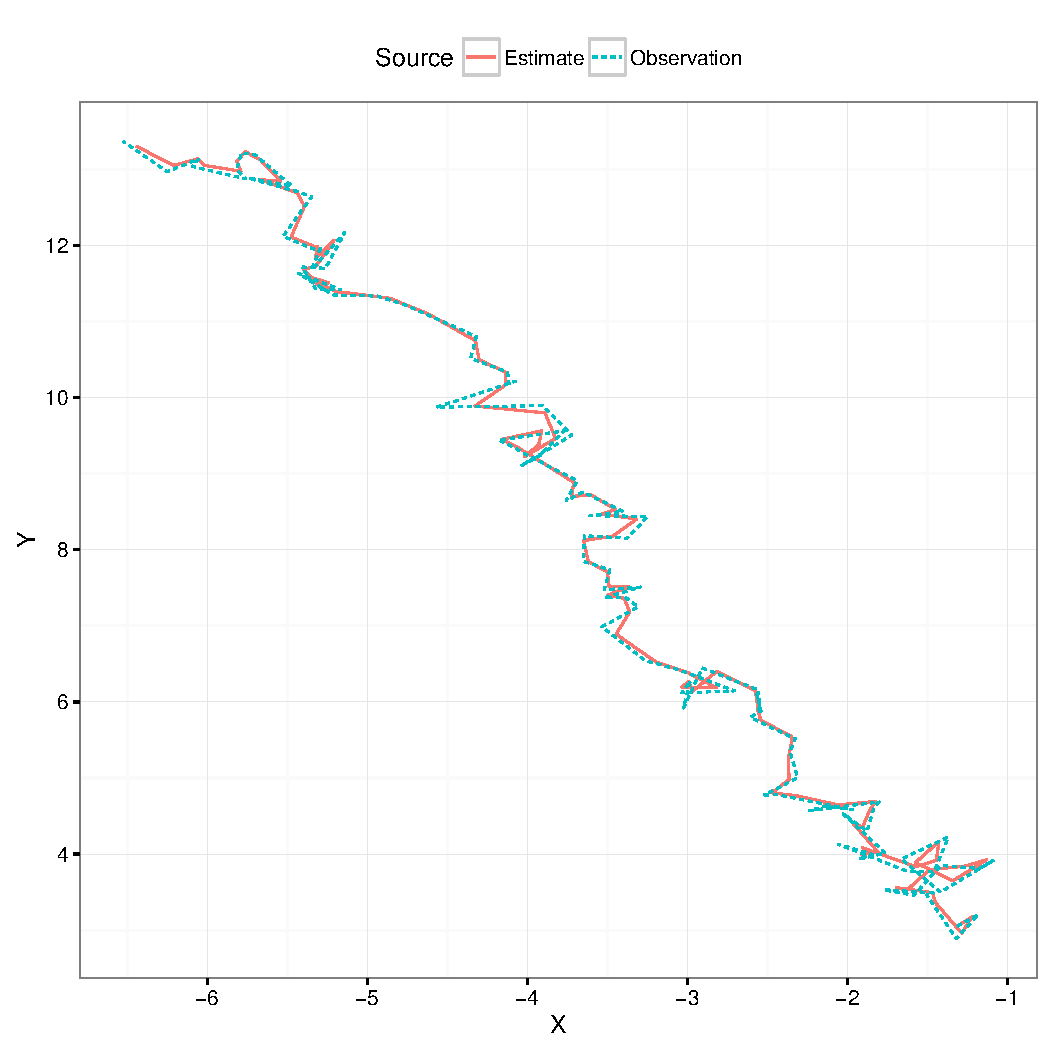
\includegraphics[width=\linewidth]{cpp/pf}
  \caption{A simple particle filter}
  \label{fig:pf}
\end{figure}

Before diving into the details of the implementation of \cppinline{PFState},
etc., we will first define a few constant and types. The state space is of
dimension $4$. And it is natural to use a \cppinline{StateMatrix} as the base
class of \cppinline{PFState},
\begin{cppcode}
  using PFStateBase = vsmc::StateMatrix<vsmc::RowMajor, 4, double>;
\end{cppcode}
The numbers of particles and data points are also defined as constants in this
simple example,
\begin{cppcode}
  static constexpr std::size_t N = 1000; // Number of particles
  static constexpr std::size_t n = 100;  // Number of data points
\end{cppcode}
Last, we define the following constants as the indices of each state component.
\begin{cppcode}
  static constexpr std::size_t PosX = 0;
  static constexpr std::size_t PosY = 1;
  static constexpr std::size_t VelX = 2;
  static constexpr std::size_t VelY = 3;
\end{cppcode}

\subsubsection{State: \texttt{PFState}}

As noted earlier, \cppinline{StateMatrix} will be used as the base class of
\cppinline{PFState}. Since the data will be shared by all particles, we also
store the data within this class. And methods will be provided to read the data
from an external file, and compute the log-likelihood $\ell(X^{(i)})$, which
accesses the data. Below the declaration of the class \cppinline{PFState} is
shown,
\begin{cppcode*}{texcomments}
  class PFState : public PFStateBase
  {
      public:
      using PFStateBase::PFStateBase;
  
      // Return $\ell(X_t^{(i)}|Y_t)$
      double log_likelihood(std::size_t t, size_type i) const;
  
      // Read data from an external file
      void read_data(const char *param);
  
      private:
      vsmc::Vector<double> obs_x_;
      vsmc::Vector<double> obs_y_;
  };
\end{cppcode*}

\subsubsection{Initialization: \texttt{PFInit}}

The initialization step is implemented as below,
\begin{cppcode}
  class PFInit
  {
      public:
      std::size_t operator()(vsmc::Particle<PFState> &particle, void *param)
      {
          eval_param(particle, param);
          eval_pre(particle);
          std::size_t acc = 0;
          for (auto sp : particle)
              acc += eval_sp(sp);
          eval_post(particle);
  
          return acc;
      }
  
      void eval_param(vsmc::Particle<PFState> &particle, void *param)
      {
          particle.value().read_data(static_cast<const char *>(param));
      }
  
      void eval_pre(vsmc::Particle<PFState> &particle)
      {
          w_.resize(particle.size());
      }
  
      std::size_t eval_sp(vsmc::SingleParticle<PFState> sp)
      {
          vsmc::NormalDistribution<double> norm_pos(0, 2);
          vsmc::NormalDistribution<double> norm_vel(0, 1);
          sp.state(PosX) = norm_pos(sp.rng());
          sp.state(PosY) = norm_pos(sp.rng());
          sp.state(VelX) = norm_vel(sp.rng());
          sp.state(VelY) = norm_vel(sp.rng());
          w_[sp.id()] = sp.particle().value().log_likelihood(0, sp.id());
  
          return 0;
      }
  
      void eval_post(vsmc::Particle<PFState> &particle)
      {
          particle.weight().set_log(w_.data());
      }
  
      private:
      vsmc::Vector<double> w_;
  };
\end{cppcode}
An object of this class is convertible to
\cppinline{Sampler<PFState>::init_type}. In the main method,
\cppinline{operator()}, \cppinline{eval_param} is called first to initialize
the data. Then \cppinline{eval_pre} is called to allocated any resource this
class need before calling any \cppinline{eval_sp}. In this case, it allocate
the vector \cppinline{w_} for storing weights computed later. Next, the main
loop initializes each state component with the respective Gaussian
distribution, computes the log-likelihood and store them in the vector
allocated in the last step. This is done by calling the \cppinline{eval_sp}
method. After all particles have been initialized, we set the weights of the
system in \cppinline{eval_post}. Later in section~\ref{sec:Symmetric
  Multiprocessing} it will become clear why we structured the implementation
this way.

\subsubsection{Move: \texttt{PFMove}}

The move step is similar to the initialization. We show the declaration here,
\begin{cppcode}
  class PFMove
  {
      public:
      std::size_t operator()(std::size_t t, vsmc::Particle<PFState> &particle);
      void eval_pre(std::size_t t, vsmc::Particle<PFState> &particle);
      std::size_t eval_sp(std::size_t t, vsmc::SingleParticle<PFState> sp);
      void eval_post(std::size_t t, vsmc::Particle<PFState> &particle);
  
      private:
      vsmc::Vector<double> w_;
  };
\end{cppcode}

\subsubsection{Monitor: \texttt{PFMEval}}

Last we define \cppinline{PFMEval}, which simply copies the values of the
positions.
\begin{cppcode}
  class PFMEval
  {
      public:
      void operator()(std::size_t t, std::size_t dim,
          vsmc::Particle<PFState> &particle, double *r)
      {
          eval_pre(t, particle);
          for (std::size_t i = 0; i != particle.size(); ++i, r += dim)
              eval_sp(t, dim, particle.sp(i), r);
          eval_post(t, particle);
      }
  
      void eval_pre(std::size_t t, vsmc::Particle<PFState> &particle) {}
  
      void eval_sp(std::size_t t, std::size_t dim,
          vsmc::SingleParticle<PFState> sp, double *r)
      {
          r[0] = sp.state(PosX);
          r[1] = sp.state(PosY);
      }
  
      void eval_post(std::size_t t, vsmc::Particle<PFState> &particle) {}
  };
\end{cppcode}

\section{Symmetric Multiprocessing}
\label{sec:Symmetric Multiprocessing}

The above example is implemented in a sequential fashion. However, the loops
inside \cppinline{PFInit}, \cppinline{PFMove} and \cppinline{PFMEval} clearly
can be parallelized. The library provides basic support of multicore
parallelization through its \smp module. Two widely used backends, OpenMP and
\tbb are available. Here we demonstrate how to use the \tbb backend. First we
will declare the implementation classes as subclasses as below,
\begin{cppcode}
  class PFInit : public InitializationTBB<PFState>;
  class PFMove : public MoveTBB<PFState>;
  class PFMEval : public MonitorEvalTBB<PFState>;
\end{cppcode}
And remove \cppinline{operator()} from their implementations. After these
changes, the implementation will be parallelized using \tbb. The complete
program can be found in section The complete program is shown in
appendix~\appref{sec:Parallelized implementation of a simple particle filter}.

It works as if \cppinline{InitializationTBB<PFState>} has an implementation of
\cppinline{operator()} as we did before, except it is parallelized. Now it is
clear that, method such as \cppinline{eval_pre} and \cppinline{eval_post} are
called before and after the main loop. Method \cppinline{eval_sp} is called
within the loop and it need to be thread-safe if called with different
arguments. This is the main reason we constructed the
\cppinline{NormalDistribution} objects within \cppinline{eval_sp} instead of as
member data, even though they are constructed in exactly the same way for each
particle. This is because \cppinline{NormalDistribution::operator()} is a
mutable method and thus not thread-safe. If any of these member functions does
not do anything, then it does not have to be defined in the derived class.

Apart from the three base classes we have shown here, there are also
\cppinline{InitializationOMP}, etc., for using the OpenMP backend. And
\cppinline{InitializationSEQ}, etc., for implementation without
parallelization. The later works in exactly the same way as our implementation
in the last section. It is often easier to debug a single-threaded program than
a parallelized one. And thus one may develop the algorithm with the sequential
backend and obtain optimal performance latter by only changing the name of a
few base class names. This can usually be done automatically through a build
system.

\subsection{Performance consideration}
\label{sec:Performance consideration}

The base classes dispatch calls to \cppinline{eval_pre}, \cppinline{eval_sp},
etc., through the virtual function mechanism. The performance impact is minimal
for \cppinline{eval_pre} and \cppinline{eval_post}, since they are called only
once in each iteration and we expect the computational cost will be dominated
by \cppinline{eval_sp} in most cases. However, the dynamic dispatch can cause
considerable performance degenerating if the cost of a single call to
\cppinline{eval_sp} is small while the number of particles is large. Modern
optimizing compilers can usually devirtualize the method calls in trivial
situations. However, it is not always possible. In this situation, the library
will need a little help from the user to make compile-time dispatch. For each
implementation class, we will declare it in the following way,
\begin{cppcode}
  class PFInit : public InitializationTBB<PFState, PFInit>;
  class PFMove : public MoveTBB<PFState, PFMove>;
  class PFMEval : public MonitorEvalTBB<PFState, PFMEval>;
\end{cppcode}
The second template argument of the base class need to be exactly the same as
the derived class. For interested users, this is called Curiously Recurring
Template
Pattern\footnote{\url{https://en.wikipedia.org/wiki/Curiously_recurring_template_pattern}}
(\crtp). This usage of the library's base classes also provides other
flexibility. The methods \cppinline{eval_pre} etc., can be either
\cppinline{const} or mutable. They can also be \cppinline{static}.
